\documentclass[tikz]{standalone}
\usetikzlibrary{shapes,arrows.meta}
\begin{document}
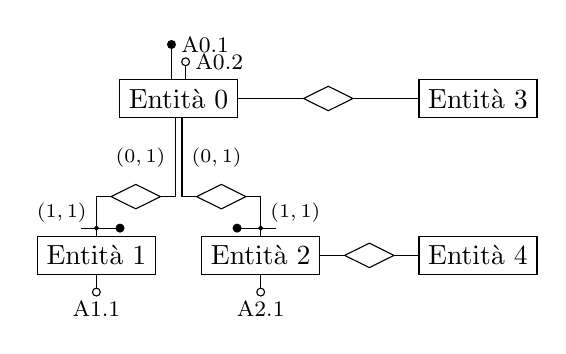
\begin{tikzpicture}
    \draw

    %%* Attributi:
    %%  node[draw, circle, inner sep=1pt,anchor=180, fill=black]{}node[right]{\footnotesize A}
    %%? Distanza orizzontale: E -(0.25,0.x)- A
    %%? Distanza verticale: E -(0,x * 0.22)- A

    %%* Cardinalità:
    %%  node[below right]{\scriptsize $(0,N)$}
    %%  node[above right]{\scriptsize $(0,N)$}
    %%  node[midway, above]{\scriptsize $(0,N)$}

    %%* Relazione:
    %%  node[draw, diamond, shape aspect=2, inner sep=3pt, anchor=90](r1){}
    %%  node[draw, diamond, shape aspect=2, inner sep=0.2pt, anchor=180](r2){R2}

    %%* Entità:
    %%  node[draw, rectangle, anchor=90](e1){}
    %%? Distanza verticale: E -(0.3)- R -(0.3) E
    %%? Distanza orizzontale: E -(0.75)- R -(0.75)- E

    (0,0)node[draw, rectangle, anchor=270](e0){Entità 0}
    (e0.110)--++(0,0.44)node[draw, circle, inner sep=1pt, fill=black]{}node[right]{\footnotesize A0.1}
    (e0.70)--++(0,0.22)node[draw, circle, inner sep=1pt, fill=white]{}node[right]{\footnotesize A0.2}


    (e0.260)--++(0,-1)node[midway, left]{\scriptsize $(0,1)$}--++(-1,0)node[fill=white, midway, draw, diamond, shape aspect=2, inner sep=3pt](r3){}--++(0,-0.4)node[midway, left]{\scriptsize $(1,1)$}node[draw, circle, inner sep=0.5pt, fill=black](a){}--++(0,-0.1)node[draw, rectangle, anchor=90](e1){Entità 1}
    (e0.280)--++(0,-1)node[midway, right]{\scriptsize $(0,1)$}--++(1,0)node[fill=white, midway, draw, diamond, shape aspect=2, inner sep=3pt](r4){}--++(0,-0.4)node[midway, right]{\scriptsize $(1,1)$}node[draw, circle, inner sep=0.5pt,fill=black](b){}--++(0,-0.1)node[draw, rectangle, anchor=90](e2){Entità 2}
    
    (a)++(-0.2,0)--++(0.5,0)node[draw, circle, inner sep=1pt, fill=black]{}    
    (b)++(0.2,0)--++(-0.5,0)node[draw, circle, inner sep=1pt, fill=black]{}


    (e1.270)--++(0,-0.22)node[draw, circle, inner sep=1pt, fill=white]{}node[below]{\footnotesize A1.1}
    (e2.270)--++(0,-0.22)node[draw, circle, inner sep=1pt, fill=white]{}node[below]{\footnotesize A2.1}

    (e2.0)--++(0.3,0)node[draw, diamond, shape aspect=2, inner sep=3pt, anchor=180](r2){}
    (r2.0)--++(0.3,0)node[draw, rectangle, anchor=180](e4){Entità 4}

    (e4.90)++(0,1.5)node[draw, rectangle, anchor=270](e3){Entità 3}
    (e0.0)--(e3.180)node[fill=white, midway, draw, diamond, shape aspect=2, inner sep=3pt](r1){}
    ;
\end{tikzpicture}
\end{document}